% ============================================================
\chapter{The Data Science Pipeline}
\label{ch:pipeline}
% ============================================================

\section{What is Data Science?}

\begin{definition}[Data Science]
\textbf{Data science} is an interdisciplinary field that uses scientific methods, algorithms, and systems to extract knowledge and insights from structured and unstructured data.
\end{definition}

\begin{intuition}
Data science sits at the intersection of three domains:
\begin{itemize}
\item \textbf{Mathematics and Statistics}: modeling, inference, probability.
\item \textbf{Computer Science}: programming, algorithms, databases.
\item \textbf{Domain Expertise}: understanding of the application area.
\end{itemize}
\end{intuition}

\begin{center}
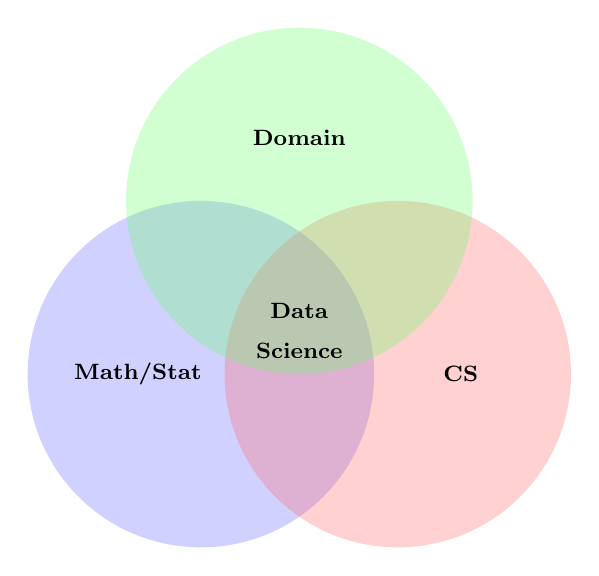
\begin{tikzpicture}
  \begin{scope}[fill opacity=0.3, text opacity=1]
    \fill[blue!60] (0,0) circle (2.2cm);
    \fill[red!60] (2.5,0) circle (2.2cm);
    \fill[green!60] (1.25,2.2) circle (2.2cm);
  \end{scope}
  \node at (-0.8,0) {\footnotesize\textbf{Math/Stat}};
  \node at (3.3,0) {\footnotesize\textbf{CS}};
  \node at (1.25,3.0) {\footnotesize\textbf{Domain}};
  \node at (1.25,0.8) {\footnotesize\textbf{Data}};
  \node at (1.25,0.3) {\footnotesize\textbf{Science}};
\end{tikzpicture}
\end{center}

\section{The Typical Pipeline}

A data science project generally follows a multi-step pipeline:

\begin{center}
\begin{tikzpicture}[
  block/.style={rectangle, draw, fill=blue!10, rounded corners,
    minimum width=2.8cm, minimum height=0.8cm, align=center, font=\small},
  arr/.style={-{Stealth[length=3mm]}, thick}
]
\node[block] (q) at (0,0) {Question};
\node[block] (d) at (3.5,0) {Data};
\node[block] (n) at (7,0) {Cleaning};
\node[block] (e) at (10.5,0) {Exploration};
\node[block] (m) at (3.5,-1.8) {Modeling};
\node[block] (v) at (7,-1.8) {Evaluation};
\node[block] (c) at (10.5,-1.8) {Communication};
\draw[arr] (q) -- (d);
\draw[arr] (d) -- (n);
\draw[arr] (n) -- (e);
\draw[arr] (e) -- (m);
\draw[arr] (m) -- (v);
\draw[arr] (v) -- (c);
\end{tikzpicture}
\end{center}

\begin{enumerate}
\item \textbf{Problem formulation}: clearly define the question.
\item \textbf{Data collection}: import from files, databases, APIs.
\item \textbf{Cleaning}: handle missing values, duplicates, errors.
\item \textbf{Exploration} (EDA): visualize and summarize the data.
\item \textbf{Modeling}: apply statistical or machine learning models.
\item \textbf{Evaluation}: measure model performance.
\item \textbf{Communication}: present results clearly.
\end{enumerate}

\section{The Python Data Science Ecosystem}

\begin{keyformulas}[title=\textbf{Essential Libraries}]
\begin{tabular}{ll}
\toprule
\textbf{Library} & \textbf{Role} \\
\midrule
\py{numpy} & Numerical computing, arrays \\
\py{pandas} & Tabular data manipulation \\
\py{matplotlib} & Basic visualization \\
\py{seaborn} & Statistical visualization \\
\py{scikit-learn} & Machine learning \\
\py{scipy} & Statistics and optimization \\
\bottomrule
\end{tabular}
\end{keyformulas}

\begin{codeblock}[title=\textbf{Python --- Installation and imports}]
\begin{minted}{python}
# Installation (in a terminal)
# pip install numpy pandas matplotlib seaborn scikit-learn

import numpy as np
import pandas as pd
import matplotlib.pyplot as plt
import seaborn as sns
from sklearn.model_selection import train_test_split
from sklearn.linear_model import LinearRegression

print(f"NumPy:   {np.__version__}")
print(f"Pandas:  {pd.__version__}")
print(f"Seaborn: {sns.__version__}")
\end{minted}
\end{codeblock}

\begin{codeoutput}
\begin{verbatim}
NumPy:   1.26.4
Pandas:  2.2.1
Seaborn: 0.13.2
\end{verbatim}
\end{codeoutput}

\section{First Complete Example: the Iris Dataset}

Let us illustrate the full pipeline on Fisher's \textbf{Iris} dataset (1936), containing 150 flower measurements across 3 species.

\begin{codeblock}[title=\textbf{Python --- Load and explore Iris}]
\begin{minted}{python}
from sklearn.datasets import load_iris

# 1. Load data
iris = load_iris(as_frame=True)
df = iris.frame
print(df.shape)
print(df.head())
\end{minted}
\end{codeblock}

\begin{codeoutput}
\begin{verbatim}
(150, 5)
   sepal length (cm)  sepal width (cm)  petal length (cm)  petal width (cm)  target
0                5.1               3.5                1.4               0.2       0
1                4.9               3.0                1.4               0.2       0
2                4.7               3.2                1.3               0.2       0
3                4.6               3.1                1.5               0.2       0
4                5.0               3.6                1.4               0.2       0
\end{verbatim}
\end{codeoutput}

\begin{codeblock}[title=\textbf{Python --- Descriptive statistics}]
\begin{minted}{python}
# 2. Explore
print(df.describe().round(2))
print(f"\nMissing values:\n{df.isnull().sum()}")
\end{minted}
\end{codeblock}

\begin{codeoutput}
\begin{verbatim}
       sepal length (cm)  sepal width (cm)  petal length (cm)  petal width (cm)  target
count             150.00            150.00             150.00            150.00  150.00
mean                5.84              3.06               3.76              1.20    1.00
std                 0.83              0.44               1.77              0.76    0.82
min                 4.30              2.00               1.00              0.10    0.00
25%                 5.10              2.80               1.60              0.30    0.00
50%                 5.80              3.00               4.35              1.30    1.00
75%                 6.40              3.30               5.10              1.80    2.00
max                 7.90              4.40               6.90              2.50    2.00

Missing values:
sepal length (cm)    0
sepal width (cm)     0
petal length (cm)    0
petal width (cm)     0
target               0
\end{verbatim}
\end{codeoutput}

\begin{codeblock}[title=\textbf{Python --- Visualization}]
\begin{minted}{python}
# 3. Visualize
fig, axes = plt.subplots(1, 2, figsize=(12, 5))

for species in [0, 1, 2]:
    subset = df[df['target'] == species]
    axes[0].hist(subset['petal length (cm)'], alpha=0.6,
                 label=iris.target_names[species], bins=15)
axes[0].set_xlabel('Petal Length (cm)')
axes[0].set_ylabel('Frequency')
axes[0].legend()

for species in [0, 1, 2]:
    subset = df[df['target'] == species]
    axes[1].scatter(subset['sepal length (cm)'],
                    subset['petal length (cm)'],
                    label=iris.target_names[species], alpha=0.7)
axes[1].set_xlabel('Sepal Length (cm)')
axes[1].set_ylabel('Petal Length (cm)')
axes[1].legend()
plt.tight_layout()
plt.savefig('ch01_iris_explore.pdf')
plt.show()
\end{minted}
\end{codeblock}

\begin{codeblock}[title=\textbf{Python --- Simple modeling}]
\begin{minted}{python}
from sklearn.neighbors import KNeighborsClassifier
from sklearn.metrics import accuracy_score

# 4. Model
X = df[['sepal length (cm)', 'sepal width (cm)',
        'petal length (cm)', 'petal width (cm)']]
y = df['target']

X_train, X_test, y_train, y_test = train_test_split(
    X, y, test_size=0.3, random_state=42)

knn = KNeighborsClassifier(n_neighbors=5)
knn.fit(X_train, y_train)
y_pred = knn.predict(X_test)

# 5. Evaluate
print(f"Accuracy: {accuracy_score(y_test, y_pred):.2%}")
\end{minted}
\end{codeblock}

\begin{codeoutput}
\begin{verbatim}
Accuracy: 100.00%
\end{verbatim}
\end{codeoutput}

\section{Types of Data Science Problems}

\begin{center}
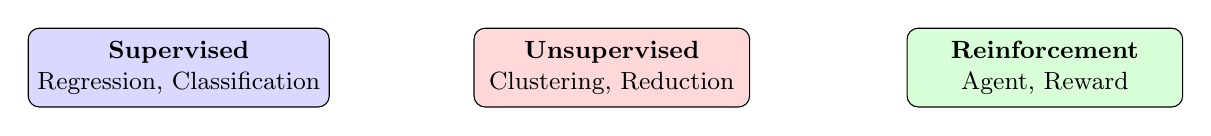
\begin{tikzpicture}[
  box/.style={rectangle, draw, fill=#1!15, rounded corners,
    minimum width=3.5cm, minimum height=1cm, align=center, font=\small},
  arr/.style={-{Stealth}, thick}
]
\node[align=center,box=blue] (sup) at (0,0) {\textbf{Supervised}\\Regression, Classification};
\node[align=center,box=red] (unsup) at (5.5,0) {\textbf{Unsupervised}\\Clustering, Reduction};
\node[align=center,box=green] (semi) at (11,0) {\textbf{Reinforcement}\\Agent, Reward};
\end{tikzpicture}
\end{center}

\begin{itemize}
\item \textbf{Supervised learning}: we have a label $y$ for each observation $\bm{x}$.
  \begin{itemize}
  \item \emph{Regression}: $y \in \R$ (predict a price, temperature).
  \item \emph{Classification}: $y \in \{0,1,\ldots,K-1\}$ (detect spam, cancer).
  \end{itemize}
\item \textbf{Unsupervised learning}: no labels, we seek structure (clusters, principal components).
\item \textbf{Reinforcement learning}: an agent learns by trial and error in an environment.
\end{itemize}

\section{Best Practices}

\begin{bestpractice}
\begin{enumerate}
\item \textbf{Reproducibility}: fix random seeds (\py{random_state=42}), version control.
\item \textbf{Train/test separation}: never evaluate on training data.
\item \textbf{Documentation}: comment code, note assumptions.
\item \textbf{Iteration}: start simple, add complexity gradually.
\end{enumerate}
\end{bestpractice}

\begin{warning}
Never look at test data before finalizing your model. \emph{Data leakage} is the most common and dangerous mistake in data science.
\end{warning}

\section{Exercises}

\begin{exercise}[$\star$]
Load the \py{load_wine()} dataset from scikit-learn. Display its dimensions, variable names, and descriptive statistics.
\end{exercise}

\begin{exercise}[$\star$]
On the Iris dataset, create a scatter plot of sepal width vs.\ sepal length, colored by species.
\end{exercise}

\begin{exercise}[$\star\star$]
Apply a $k$-nearest neighbors classifier to the Wine dataset with $k=3,5,7$. Compare accuracies on a 30\% test set.
\end{exercise}

\begin{exercise}[$\star\star$]
Write a function \py{full_pipeline(dataset, k)} that loads a scikit-learn dataset, splits into train/test, trains a KNN with $k$ neighbors, and returns the accuracy.
\end{exercise}

\begin{keyformulas}[title=\textbf{Chapter Summary}]
\begin{itemize}
\item Data science follows a pipeline: Question $\to$ Data $\to$ Cleaning $\to$ Exploration $\to$ Modeling $\to$ Evaluation $\to$ Communication.
\item The Python ecosystem provides powerful tools: \py{pandas}, \py{matplotlib}, \py{scikit-learn}.
\item Three major families: supervised, unsupervised, reinforcement.
\item Golden rules: reproducibility, train/test separation, start simple.
\end{itemize}
\end{keyformulas}
